\chapter{Dizajn}


Za unos neophodnih ulaznih parametara potrebnih za  proračune kod distantne zaštite, kao i za vizualizaciju rezultata i veličina bitnih za detekciju kvara koristili smo \textit{MATLAB}-ov GUI (eng. \textit{\textbf{G}raphical \textbf{U}ser \textit{I}nterfaces}). Pomoću njega možemo na jednostavniji i efikasniji način prikupiti set potrebnih ulaznih podataka i prikazati rezultate.


Slikom \ref{fig:GUI} prikazan je primjer izgleda GUI-a za slučaj dvofaznog kratkog spoja. GUI  se sastoji od šest dijelova koji su zaduženi za unos i obradu karakterističnih veličina. U nastavku ćemo opisati svaki od njih.

\begin{figure}[H]
  \centering
  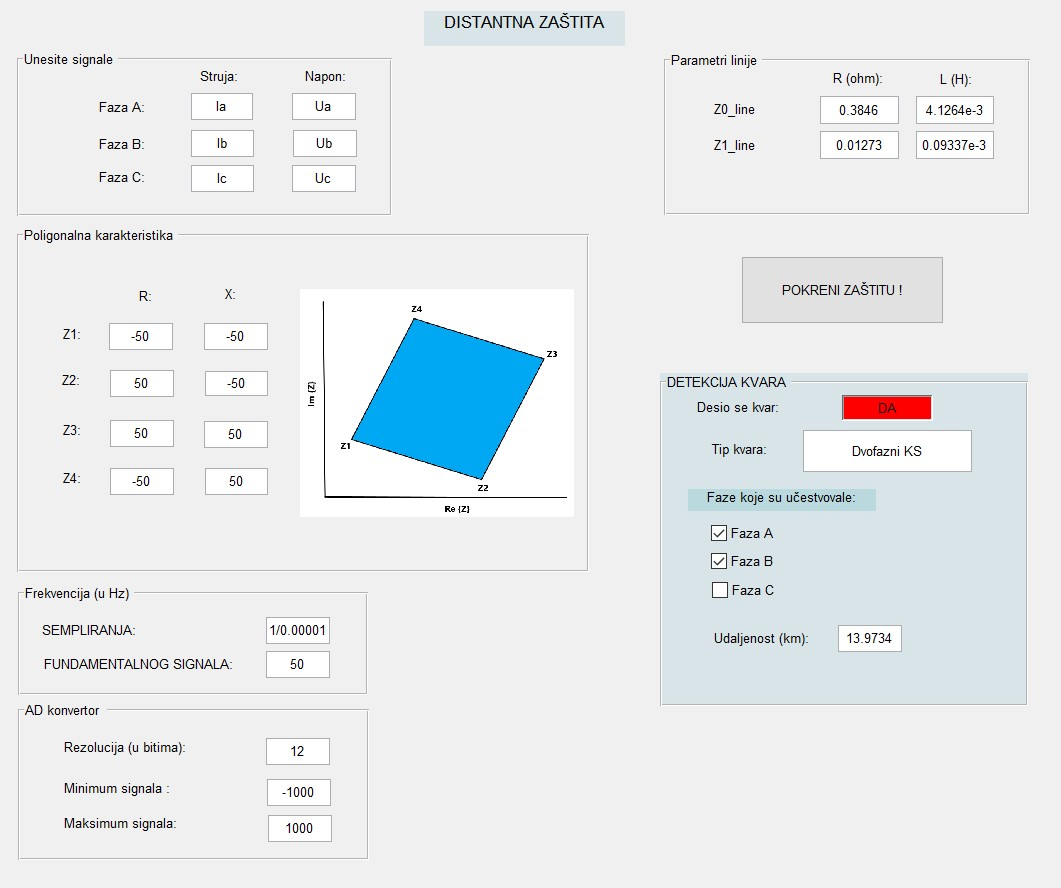
\includegraphics[width=1\textwidth]{GUI}
  \caption{Distantna zaštita - razvijeni GUI}
  \label{fig:GUI}
\end{figure}


Prvo će biti navedeni ulazni parametri zaštite koje unosi odgovorna osoba.

U prvom dijelu pod nazivom \textbf{„Unesite signale“} , unosimo varijable struja $I_a, I_b, I_c$ i napona $U_a, U_b, U_c$ za svaku od faza čije ćemo vrijednosti koristiti. Te vrijednosti učitavamo iz workspace-a u formi vektora dimenzija $1xN$ gdje je N broj uzoraka datih signala. 
U drugom dijelu, pod nazivom \textbf{„Poligonalna karakteristika“}, unosimo realne i imaginarne vrijednosti impedansi koje čine poligon, pri tome poštujući raspored prikazan na slici ($Z_1$-donja lijeva, $Z_2$-donja desna, $Z_3$-gornja desna, $Z_4$- gornja lijeva). Važno je napomenuti, da vrijednosti impedansi koje čine poligon budu u skladu sa posmatranom mrežom što bi značilo da zaštita u slučaju kada nema kvara ne smije da proradi. 


U trećem dijelu, pod nazivom \textbf{„Frekvencija“} unosimo frekvenciju sempliranju i frekvenciju fundamentalnog signala u (Hz).

U četvrtom dijelu, pod nazivom \textbf{„AD konvertor“} unosimo rezoluciju u bitima, minimalnu i maksimalnu  vrijednost signala.

U petom dijelu, pod nazivom \textbf{„Parametri linije“} unosimo realne i imaginarne vrijednosti podužne impedanse nulte i pozitivne komponente, koje odgovaraju liniji koja se štiti i služe kako bi se izračunala udaljenost na kojoj se desio eventualni kvar. 

\vspace{0.5cm}
\begin{center}
    * * *
\end{center}

\vspace{0.5cm}

Da bi smo pokrenuli simulaciju za detekciju kvara potrebno je da pritisnemo na odgovarajuće dugme pod nazivom \textbf{ „Pokreni zaštitu!“}.


U posljedenjem dijelu, pod nazivom \textbf{„Detekcija kvara“} dobijamo informacije da li se desio kvar( u vidu signalizacije DA (crvena boja) ili NE (zelena boja), tip kvara(jednofazni kratki spoj, dvofazni kratki spoj,trofazni kratki spoj ), faze( A  i/ili  B  i/ili  C) koje su učestvovale u kvaru i na kojoj udaljenosti(izraženoj u kilometrima). Ovim dobijamo sve potrebene informacije i detalje o nastalom kvaru.


